\outline{1}{The Duration of Reaching Movement is Longer than Predicted by Minimum Variance}
\chapter{The Duration of Reaching Movement is Longer than Predicted by Minimum Variance}
\label{cha:movementtime}


\section{Abstract}
Whether the central nervous system minimizes variability or effort in planning arm movements can be tested by measuring the preferred movement duration and endpoint variability. Here we conducted an experiment in which subjects performed arm reaching movements without visual feedback in fast-, medium-, slow-, and preferred-duration conditions. Results show that 1) total endpoint variance was smallest in the medium- duration condition and 2) subjects preferred to carry out movements that were slower than this medium-duration condition. A parsimonious explanation for the overall pattern of endpoint errors across fast, medium, preferred, and slow movement durations is that movements are planned to minimize effort as well as endpoint error due to both signal-dependent and constant noise.

This work was published at \textit{Journal of Neurophysiology} on August 24th, 2016, collaborators are Yupeng Xiao\footnote{\textit{Neuroscience Graduate Program, University of Southern California, Los Angeles, California}}, Etienne Burdet\footnote{\textit{Bioengineering Department,Imperial College, London, United Kingdom}}, James Gordon\footnote{\label{bknpt}\textit{Biokinesiology and Physical Therapy, University of Southern California, Los Angeles, California}}, and Nicolas Schweighofer\footnotemark[\ref{bknpt}]. Nicolas Schweighofer is the corresponding author. Yupeng Xiao shares the first authorship with Chunji Wang, the writer of this thesis. This chapter reprints the original published paper with permission from Chunji Wang and Nicolas Schweighofer.

\outline{2}{Introduction}
\section{Introduction}

Although most motor tasks can be carried out in an infinite number of ways with our redundant musculoskeletal system, arm movements exhibit striking regularities. 
In particular, the durations of reaching movements vary systematically with the amplitudes and the directions of movements \cite{Gordon1994}. 
According to the optimal control theory of human motor control (e.g., \cite{Flash1985, Hoff1994, Uno1989}), these regularities correspond to the minimum of a cost function that the central nervous system (CNS) considers in planning motion. Despite much research on this topic, however, it is still unclear how the CNS determines the duration of movement during planning. The stochastic optimal control model of Harris and Wolpert (1998, 2006) proposes that the CNS determines movement planning by minimizing the movement endpoint variability due to signal-dependent noise. Although this model successfully predicts trajectories and durations of saccadic eye movements and planar arm reaching movements, it is not clear whether movement endpoint variability or effort is minimized. Indeed, mathematically, the expression of movement endpoint error due to signal-dependent noise in the motor commands and the expression of effort are equivalent \cite{OSullivan2009}.

Minimizing effort (or, equivalently, minimizing endpoint variability due to signal-dependent noise) will slow down planar movements, because the torques necessary to move the arm decrease with an increase in movement duration\footnote{The rigid body dynamics $\tau = M(q)\ddot{q} + C(q,\dot{q})\dot{q}$, where $M$ is the inertia matrix and $C$ represents the Coriolis and centrifugal forces and is a quadratic function of the velocity. As the velocity decreases linearly with movement duration and the acceleration decreases quadratically, the torques required to move the arm decrease in a quadratic fashion with an increase in movement duration. Assuming that effort is, e.g., a quadratic or linear function of these torques, this implies that the effort will decrease at least cubically \cite{Shadmehr2016} with a linear increase of the movement duration.}. 
For instance, movements performed by the right hand to leftward targets are slower than movements to rightward targets \cite{Gordon1994,Park2016}. This can be attributed to greater effort (or equivalently signal-dependent noise) for leftward targets because of greater inertia at the hand for these movements \cite{Cos2011, Guigon2007, Schweighofer2015}. 

In addition to signal-dependent noise, motor commands are also corrupted by constant noise \cite{VanBeers2007, VanBeers2004}. Although such constant noise was not considered in the models of \cite{Harris1998, Harris2006} and of \cite{OSullivan2009}, it can be quite substantial. For instance, by fitting the endpoint distributions generated by simulated arm movements to actual data, van Beers et al. \cite{VanBeers2004} estimated that the standard deviation of constant noise is about twice that of signal-dependent noise. 
Minimizing variability due to constant noise shortens the movement, because variability due to this type of noise increases with movement duration (see Fig. 1 in \cite{Todorov2005} for simulation results of the respective effects of signal-dependent and constant noise for varying durations of arm movements). 
Thus minimizing variability due to both signal-dependent and constant noise would yield a minimum that could determine movement duration. 
Correspondingly, our first hypothesis is that the CNS chooses intermediate reaching movement durations to minimize endpoint variability in the face of signal-dependent and constant noise.

While minimizing endpoint variability due to both signal-dependent and constant motor noise would be sufficient to determine the duration of movements, the results of \cite{Burdet2001}  suggest that effort minimization contributes to movement planning in addition to noise. 
In that experiment, training arm reaching movements in a divergent force field led to reduced endpoint variability by increasing cocontraction of antagonist muscles. If the CNS only minimized endpoint variability, then it would use this energetically costly cocontraction strategy to reduce endpoint error \cite{Osu2004}. The fact that habitual movements (performed without force field) yield more relaxed muscle activity than in the experiment of \cite{Burdet2001} suggests that the CNS also minimizes effort. 
Minimization of effort independently from minimization of endpoint variability due to signal-dependent and constant noise sources would lengthen movement duration.

Our second hypothesis is therefore that the CNS chooses intermediate durations that are longer than those minimizing variability. 
To test these two hypotheses and examine how humans select movement durations, we conducted an arm movement experiment without visual feedback and measured endpoint variability in movements of four duration conditions, fast, medium, slow, and preferred, in which subjects choose to move at their preferred speed. The results verify our hypotheses, providing evidence for the concurrent minimization of effort and variability due to signal-dependent and constant motor noise.

\outline{2}{Methods}
\section{Methods}
Eleven young adult right-handed volunteers (between 20 and 30 years old; 3 women, 8 men) with no declared neurological impairments gave written informed consent to participate in the experiment described below, approved by the University of Southern California Ethics Committee.

Subjects performed reaching movements with their right arms to one of two targets at \ang{45} and \ang{135} (relative to the rightward direction parallel to the body) without online visual feedback in four conditions: preferred, fast, medium, and slow (Figure \ref{fig:mt-experiment}, A and C).  
Hand movements were recorded via a digital pen moving on a tablet (Wacom Tech). 
The tablet height was positioned such that the arm was moving approximately in a two-dimensional horizontal plane, with movements primarily involving horizontal shoulder and elbow rotations. 
The home position was placed such that the shoulder formed approximately a \ang{45} angle with the coronal plane and the elbow angle at \ang{90}. 
The distance from home position to targets was 7.4 cm. 
Target directions (\ang{45} and \ang{135}) were selected to maximize the difference in inertia at the hand (see Gordon et al. 1994). 
To minimize fatigue due to the large number of trials, the forearm was supported with a sling attached to a $\sim$4-meter-long cable hanging from the ceiling. 
Because of the long cable length, the pendulum effect was small.

At the beginning of each trial, subjects saw the home position, the target, and the cursor presented on a computer screen facing the subjects. 
Subjects were instructed to keep the cursor within the home position, and to move toward the target after a “go” signal at which moment all visual feedback was cleared. 
Final cursor position was displayed for 1 second after the recording period (900 ms for fast, 1,400 ms for intermediate, 2,400 ms for preferred and slow movement conditions). 
In the preferred condition, subjects reached for the targets as accurately as possible using their own selected movement duration (they were instructed to “reach naturally”). 
In the fast, medium, and slow conditions, subjects reached for the targets quickly ($\sim$350 ms), at a medium speed (400--800 ms), and slowly ($\sim$1,200 ms), respectively (Figure \ref{fig:mt-experiment} B). 
When the movement duration was outside of the range, a “too fast” or “too slow” message was displayed and the trial was repeated.
 
\begin{figure}
	\centering
	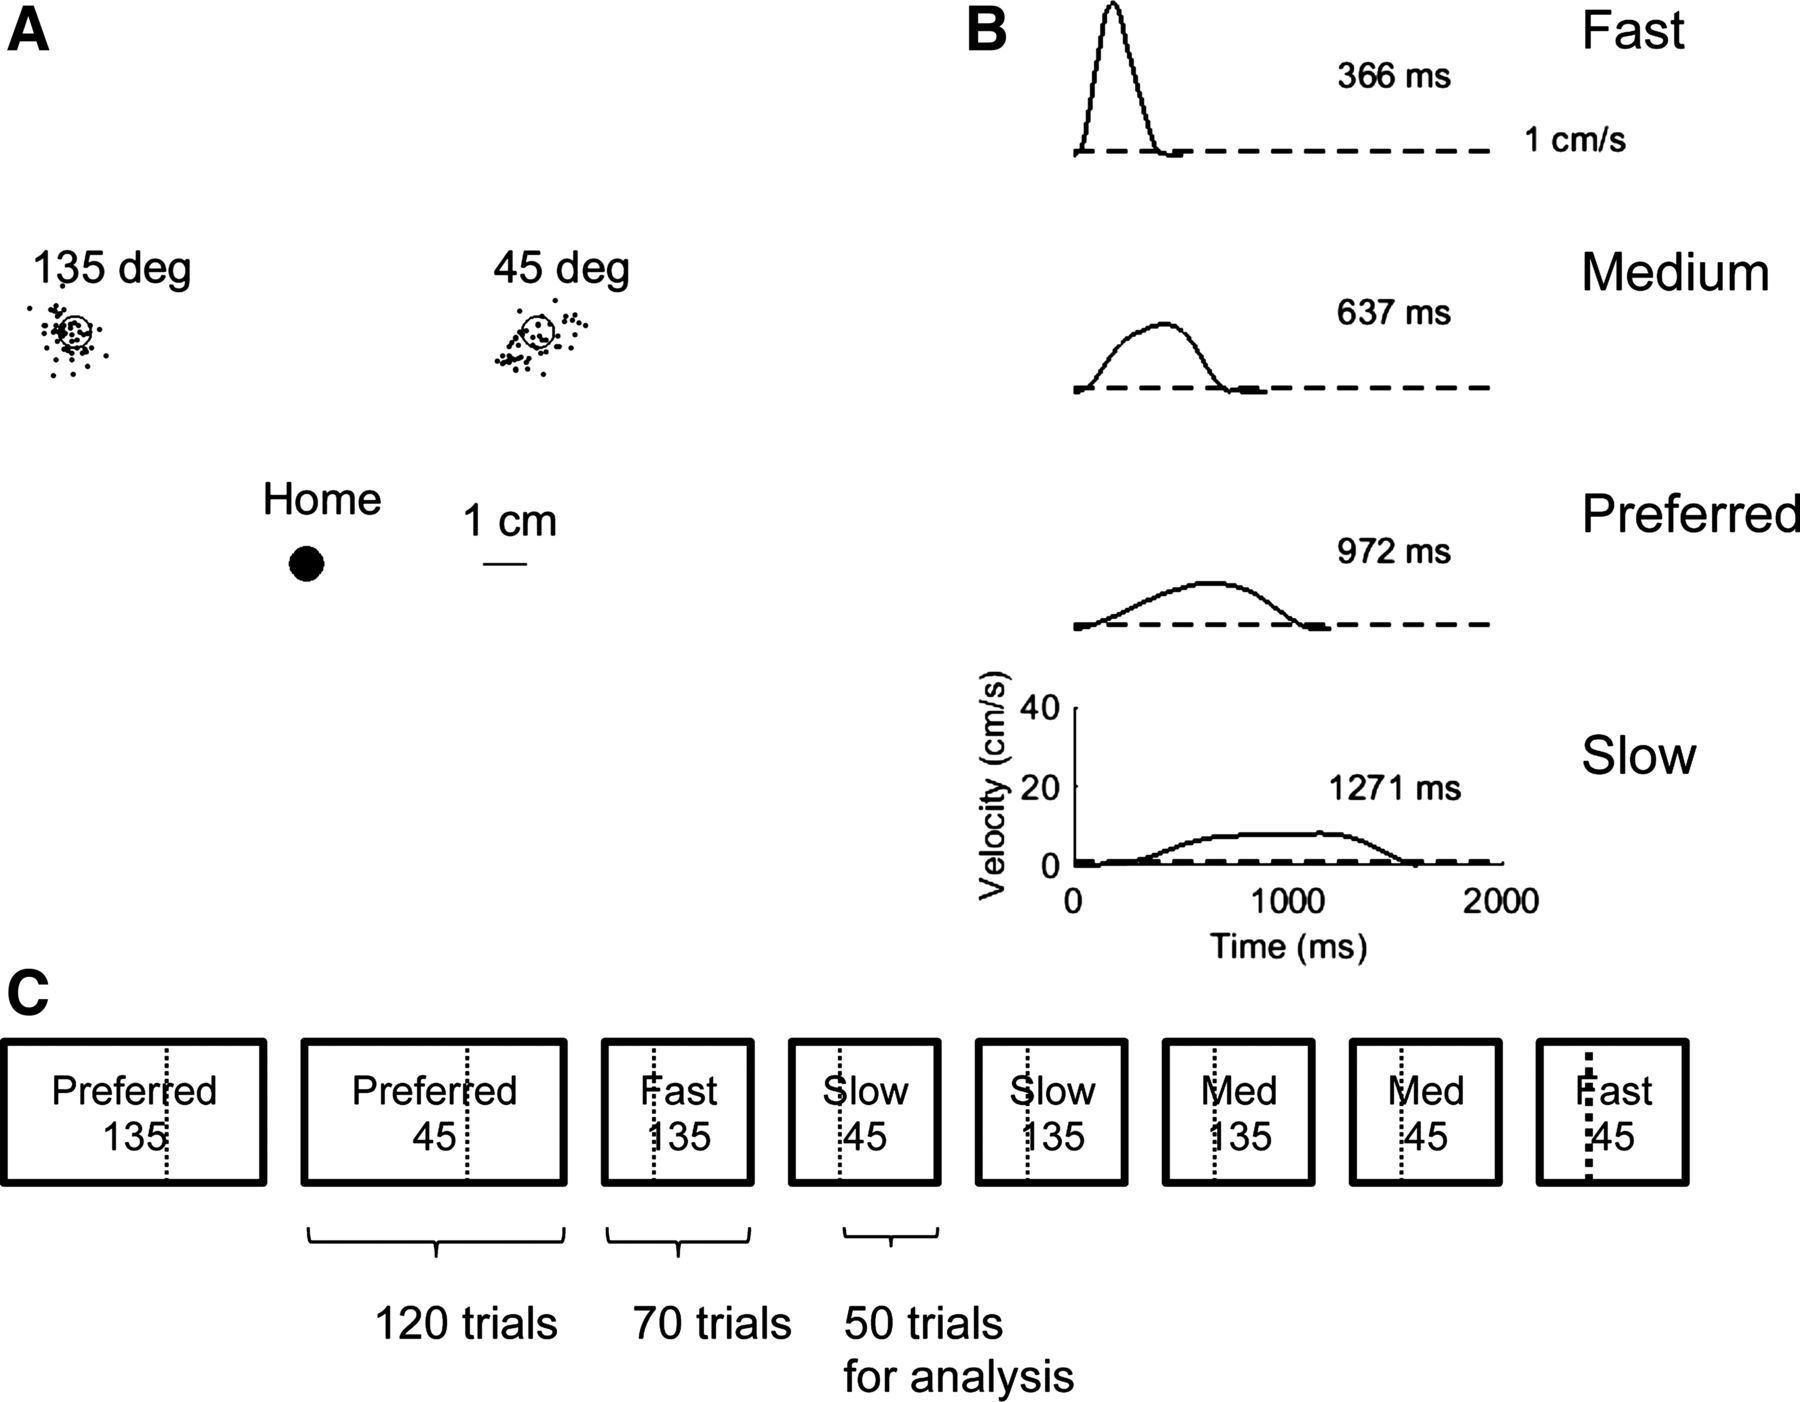
\includegraphics[width=0.8\linewidth]{figures/MT-experiment}
	\caption[Methods overview]{Methods overview. A: subjects performed horizontal reaching movements without online visual feedback to \ang{45} and \ang{135} targets in 4 duration conditions: preferred, fast, medium, and slow. The black dots around the targets show end points for 1 subject in the preferred condition. For each condition and each target, we measured endpoint variability from the variance of the endpoint distribution. B: example of velocity profiles in the 4 conditions: preferred, fast, medium, and slow. The movement duration was determined via a tangential velocity threshold of 1 cm/s. C: timeline of the experiment: example of the schedule for 1 subject. The 2 preferred movement blocks were always given first to avoid biasing the preferred duration by other conditions (the order of the 2 blocks were counterbalanced across subjects). The other 6 blocks (3 conditions, 2 targets) were then given, with the order counterbalanced for targets and conditions. Only the last 50 trials of each block (shown by dotted line) were analyzed, to remove possible initial drift and carryover in movement duration at the beginning of the blocks.}
	\label{fig:mt-experiment}
\end{figure}

Subjects first practiced all conditions in a familiarization session with online visual feedback of the cursor position, with 25 trials in each condition. 
To avoid possible carryover effects, the preferred movement duration condition was performed first, with the order of the two targets counterbalanced across subjects (Figure \ref{fig:mt-experiment} C). 
Subjects performed 120 trials for each target in the preferred condition and then 80 trials in the other six conditions (3 movement durations, fast, medium, slow for both targets), which were counterbalanced across subjects. 
The numbers of trials were determined in a pilot study, in which we noted that movement duration and final error stabilized only after a few dozen trials and that more trials were needed in the preferred condition for this stabilization to occur. 
This was confirmed in preliminary mixed-model analysis of the actual experiment, which showed a significant effect of a trial covariate on movement duration when all trials were considered. This effect disappeared (P $>$ 0.05) when only the last 50 trials in each condition and target were analyzed. Thus, for each subject, 400 movements were analyzed (50-trial block for each target in the 4 duration conditions).

Endpoint variance was computed by the trace of the covariance matrix of the endpoint distribution (Figure \ref{fig:mt-experiment} A). Because total endpoint variance was highly right-skewed, we analyzed the natural logarithm of total variance, which was approximately normal, as shown by both absolute values of skewness and kurtosis $<$ 2. Movement duration (MD) was computed with a velocity threshold of 1 cm/s across all conditions (Figure \ref{fig:mt-experiment} B).

We report the estimates of fixed effect parameters. MD and mean logarithm of variance were analyzed with mixed-effect models, with condition (fast, medium, preferred, and slow) and target (\ang{45} and \ang{135}) and their interaction as fixed effects and subjects as random intercepts. Bonferroni corrections were used for multiple comparisons. We used SPSS 18 with Restricted Maximum Likelihood method for these statistical analyses.

\outline{2}{Results}
\section{Results}

Mixed-model analysis shows significant fixed effects of condition and target on MD (both with P $<$ 0.0001) as well as a significant condition $\times$ target interaction (P $<$ 0.0001; Figure \ref{fig:mt-data} A). Overall, the subjects’ preferred MDs were longer than the medium MD and shorter than the slow MD (Figure \ref{fig:mt-data} A; P $<$ 0.0001). In addition, MD was overall smaller for targets at \ang{45} compared with targets at \ang{135} (Figure \ref{fig:mt-data} A). Individual comparisons with Bonferroni corrections show that MD was shorter for the target at \ang{45} compared with the target at \ang{135} for the fast condition (P = 0.003), the slow condition (P = 0.006), and the preferred condition, for which the difference was the largest (967 ms vs. 1,077 ms, P $<$ 0.0001). The difference between MD for the \ang{45} and \ang{135} targets was not significantly different for the medium condition (P = 0.097). 

\begin{figure}
	\centering
	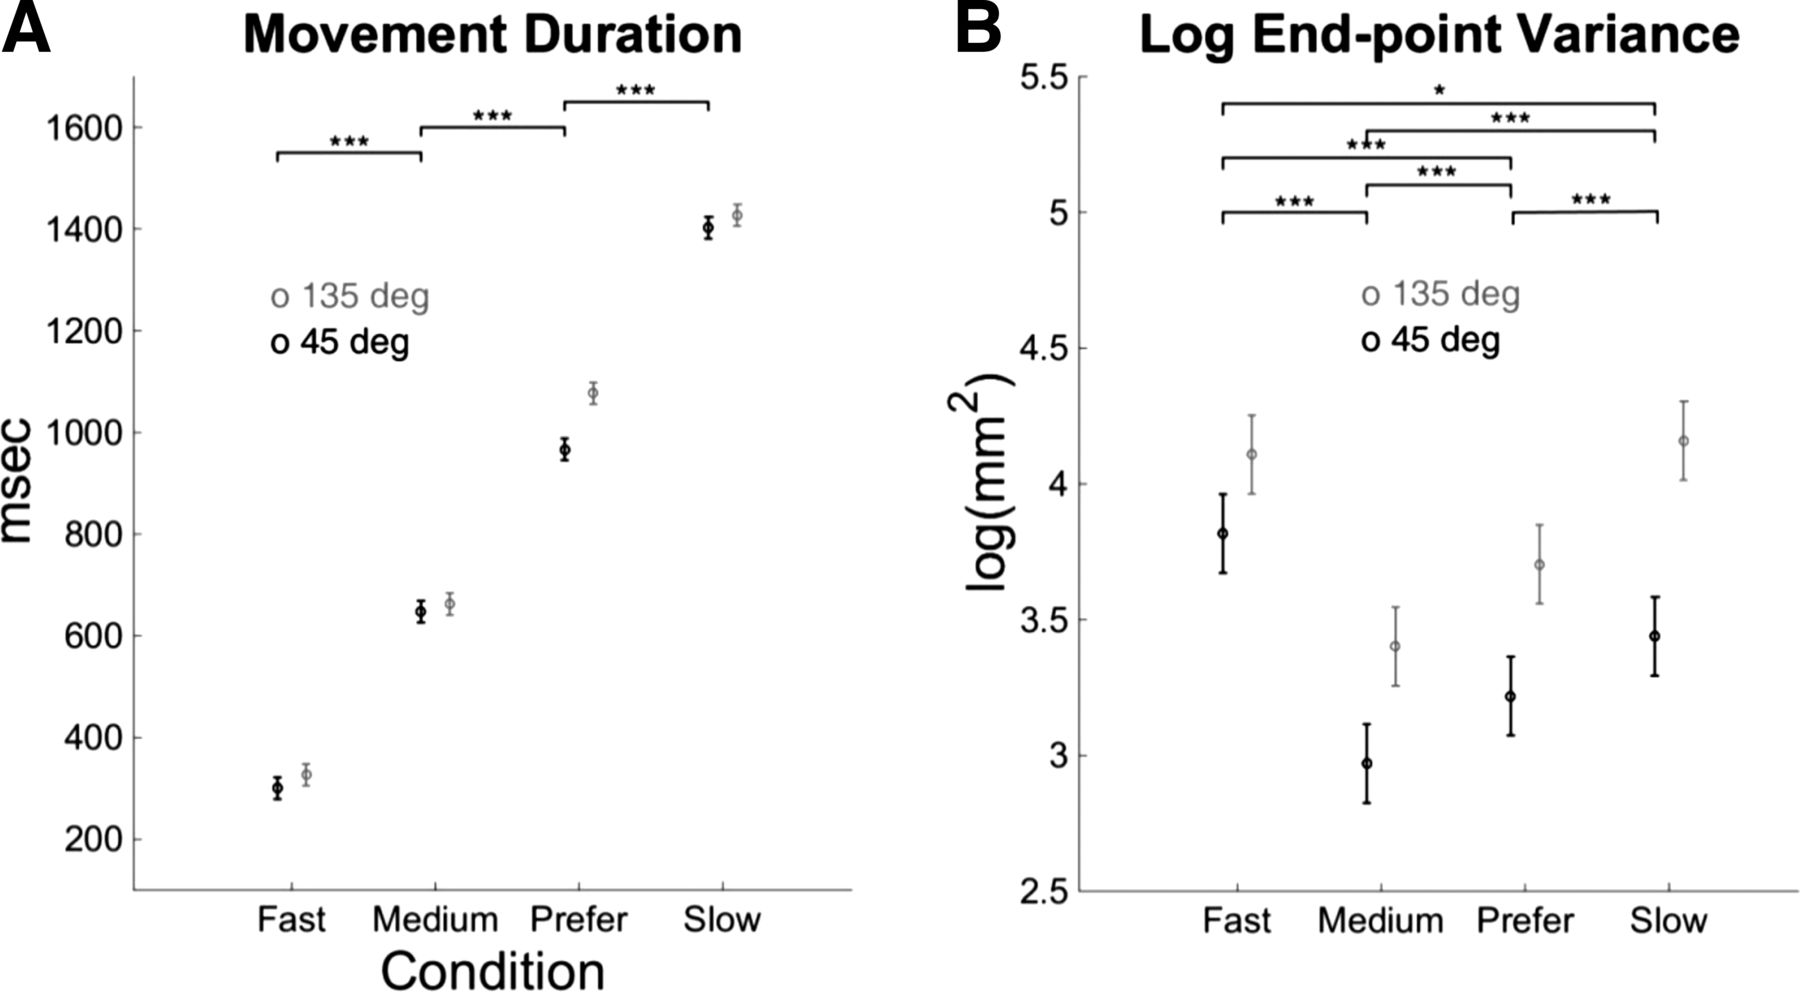
\includegraphics[width=0.8\linewidth]{figures/MT-data}
	\caption[Movement duration and endpoint movement variability]{Movement duration and endpoint movement variability in each condition for the \ang{45} and \ang{135} targets across subjects. A: movement duration in the 4 conditions for both targets. B: natural logarithm of endpoint variance in the 4 conditions for both targets. Both panels show estimated fixed effect coefficients with their confidence intervals in a model using mixed models with condition and target as main effects and target × condition interactions; see text for details. Asterisks show significance of difference between conditions for both targets (Bonferroni corrected): *P $<$ 0.05, ***P $<$ 0.0005; see text for additional comparison results.}
	\label{fig:mt-data}
\end{figure}


Mixed-model analysis shows significant fixed effects of condition and target on the (logarithm of) total endpoint variance (both with P $<$ 0.0001) as well as a significant condition $\times$ target interaction (P = 0.003). Endpoint variance was lowest for the medium duration (Figure \ref{fig:mt-data} B). Notably, for both targets, total endpoint variance in the medium movement duration condition was smaller than that in the preferred condition (P $<$ 0.0001). Total variance in the fast condition was greater than in the three other conditions (P$<$0.0001, P$<$ 0.0001, and P = 0.029 for medium, preferred and slow conditions, respectively). Variance in the slow condition was greater than variance in the preferred and medium conditions (P $<$ 0.0001 for both).

For all conditions, variance was greater for the \ang{135} target
than for the \ang{45} target (all P $<$ 0.0001). For the \ang{45} target, all differences between conditions were significant (P $<$ 0.0001), except for variance between fast and slow conditions, for which P = 1. For the \ang{135} target, all differences were significant at P $<$ 0.001, except for the differences between preferred and medium, which was significant at P = 0.015, and between preferred and slow, which was significant at P = 0.027.

\outline{2}{Discussion}
\section{Discussion}

It has long been known that the duration of arm movements has an effect on endpoint variability \cite{Fitts1954, Woodworth1899}, but the relationship had not been systematically characterized. The present study provides two valuable additions to our understanding of movement planning.

First, our results show that, in arm reaching movement without visual feedback, an intermediate movement duration minimizes endpoint variability. Such minimum of endpoint variability was previously found in saccadic movements \cite{VanBeers2008} but, to our knowledge, not in arm reaching movements. Kinematic variability in human motion originates from a number of sources \cite{Faisal2008} (Faisal et al. 2008). In particular, the noise in individual motor neurons is well approximated by signal-dependent noise (see rationale in \cite{Harris1998}). However, noise in the final motor command departs from signal-dependent noise because this aggregate command combines the activities of many motor neurons distributed over multiple muscles. It is in particular possible that cocontraction yields a departure from signal-dependent noise. As a result, studies aimed at identifying the properties of noise in the motor commands of saccades \cite{VanBeers2007} and arm movements \cite{VanBeers2004} found that the noise is best characterized as a combination of signal-dependent noise and constant noise, with constant noise making a substantial contribution. With these two sources of noise, signal-dependent noise increases endpoint variability for short movement durations and constant noise increases variability for long movement durations by inducing a drift in final position.

The variability in task execution caused by the inherent noisiness of the neuromuscular system can be reduced by feedback mechanisms. In our experiment, movements were performed without vision, and thus only proprioceptive feedback was available to the subjects. 
The effect of proprioceptive feedback on movements appears small for movements at normal speed (see, e.g., Fig. 4 in \cite{Franklin2007}). However, for slower movements the effect of such feedback on endpoint error may become more important, especially with vision. Future work will be needed to compare variability with and without vision at different and self-chosen speed.

Second, our results show that the durations of reaching movements chosen by our subjects were longer than the durations minimizing endpoint variance. Thus, unlike what has been suggested for arm movements [Harris and Wolpert 1998, 2006], natural movements without vision at self-selected speed do not minimize variance. The longer preferred durations than the duration that minimizes variance may be due to effort minimization, which tends to lengthen movement duration. Our between-target results, as well as those from previous studies (e.g., Gordon et al. 1994; Park et al. 2016) showing that subjects slowed down for movements toward the \ang{135} target, which require greatest (estimated) effort because of greater inertia at the hand (see \cite{Schweighofer2015}), are consistent with this view.

We therefore propose that movement duration is determined by minimizing both variability and effort in the context of signal-dependent noise and constant noise in the motor command. In optimal control models of movements, the duration is determined to minimize antagonistic factors. In previous models, effort and signal-dependent noise were considered as factors to lengthen movement duration, and cost of time \cite{Hoff1994} and temporal discounting \cite{Haith2012, Rigoux2012, Shadmehr2010} were considered as a factor to shorten it. However, if we consider that constant noise is responsible for greater variability in slow movements, no additional factor is needed to shorten movement time. Instead, using a combination of signal-dependent noise and constant noise, simultaneous minimization of effort and endpoint variability provides a parsimonious mechanistic explanation for the overall pattern of errors across the fast, medium, preferred, and slow movement durations. In future work, estimating effort for different targets and speeds via quantification of metabolic costs (e.g., \cite{Huang2012}) will be necessary to determine whether the minimization of variability and effort is sufficient to determine movement time.

